\documentclass{article}
\usepackage[utf8]{inputenc}
\usepackage{enumitem}
\usepackage{amsmath}

\title{Image and Video Processing Lab 1}
\author{Philine Witzig}
\date{September/October 2020}

\usepackage{natbib}
\usepackage{graphicx}
\usepackage{subcaption}

\begin{document}

\maketitle

General notes: when running the matlab script, you will be asked to enter the number of the task you want to test. Enter the numbers $1$ to $7$ in order to test the respective task. All subtasks will be executed.
\section{Images and Color Tables}
\begin{enumerate}
    \item Images are read with matlab's imread(). For truecolor images, the image itself is returned. For colormaps, we get an index matrix as well as the colormap.
    \item For converting the images to grayscale, the matlab function rgb2gray() was used. The function works for, both, truecolor images or colormaps. For the later, you simply pass the colormap itself. The function imcomplement() inverted the grayscale images then. In the complement of a grayscale or color image, each pixel value is subtracted from the maximum pixel value, i.e. 255. Cf. Figure \ref{fig:gray} for the respective results.
    \begin{figure}
        \centering
        \begin{subfigure}[c]{0.45\textwidth}
            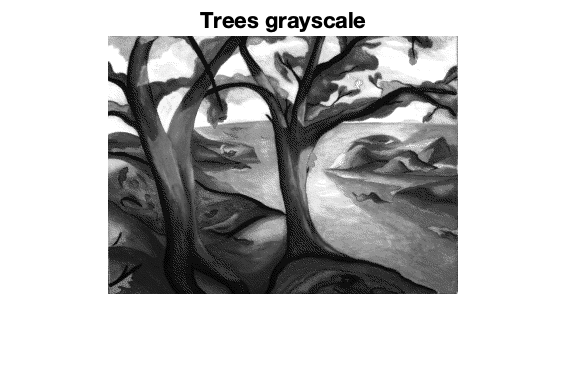
\includegraphics[width=\textwidth]{images/trees_gray.png}
            \subcaption{trees.tif in grayscale}
        \end{subfigure}
        \hfill
        \begin{subfigure}[c]{0.45\textwidth}
            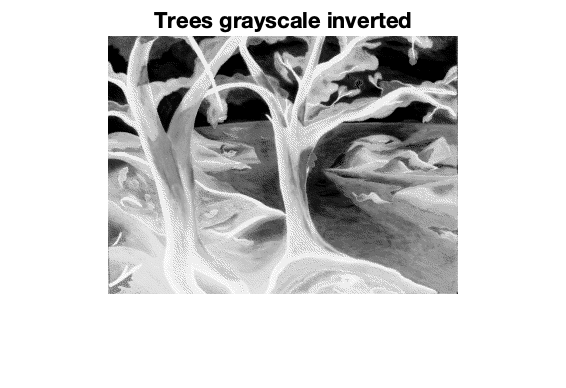
\includegraphics[width=\textwidth]{images/trees_gray_inv.png}
            \subcaption{trees.tif in grayscale, then inverted}
        \end{subfigure}
        \hfill
        \begin{subfigure}[c]{0.45\textwidth}
            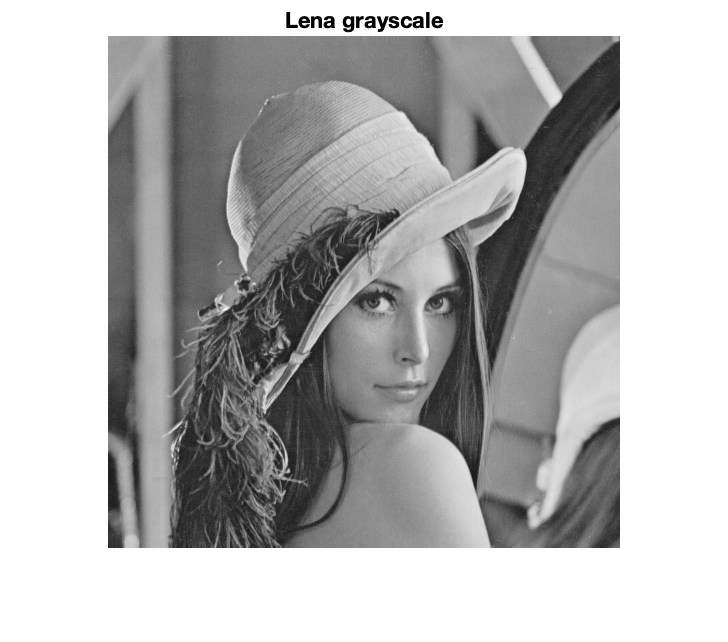
\includegraphics[width=\textwidth]{images/lena_gray.png}
            \subcaption{lena.tif in grayscale}
        \end{subfigure}
        \hfill
        \begin{subfigure}[c]{0.45\textwidth}
            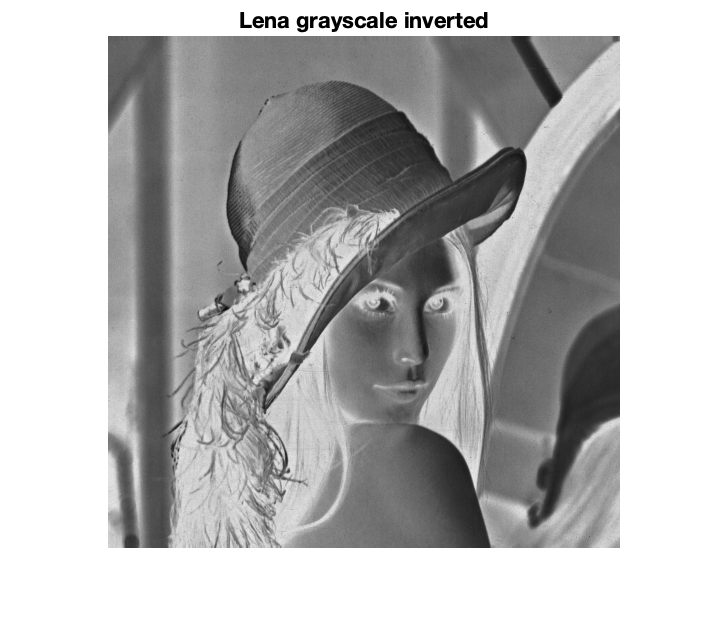
\includegraphics[width=\textwidth]{images/lena_gray_inv.png}
            \subcaption{lena.tif in grayscale, then inverted}
        \end{subfigure}
        \caption{.tif images converted to grayscale and then inverted.}
        \label{fig:gray}
    \end{figure}
    
    \item For the gamma correction, see the custom function gamma\_corr() at the bottom of the script. It modifies each channel of a colormap or a truecolor image by taking it to the power of some passed $\gamma$. The gamma correction was tested for all $\gamma \in \{0.5, 0.75, 1.25, 1.5, 1.75, 2.0\}$. In Figure \ref{fig:gamma}, one can clearly see that for $\gamma < 1$, the image and especially dark regions will become brighter, while for $\gamma > 1$, shades will become darker. Thus, gamma correction is used for manipulating the luminance of an image.
    \begin{figure}
        \centering
        \begin{subfigure}[c]{0.32\textwidth}
            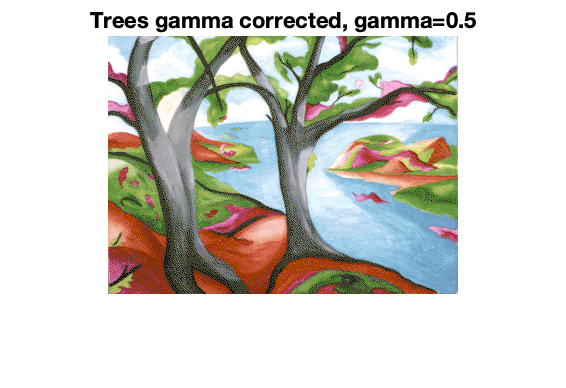
\includegraphics[width=\textwidth]{images/trees_gamma_05.png}
            \subcaption{$\gamma = 0.5$}
        \end{subfigure}
        \begin{subfigure}[c]{0.32\textwidth}
            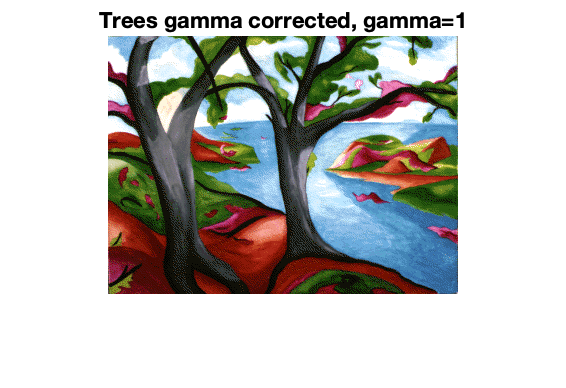
\includegraphics[width=\textwidth]{images/trees_gamma_1.png}
            \subcaption{Original}
        \end{subfigure}
        \begin{subfigure}[c]{0.32\textwidth}
            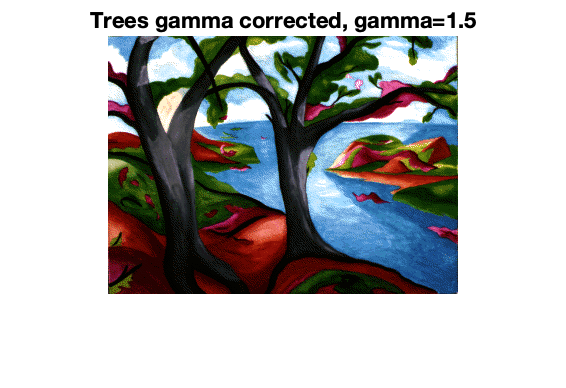
\includegraphics[width=\textwidth]{images/trees_gamma_15.png}
            \subcaption{$\gamma = 1.5$}
        \end{subfigure}
        \caption{Gamma correction on tree.tif for different $\gamma$.}
        \label{fig:gamma}
    \end{figure}
    
    \item The requested chess board will be saved in the 'Images' folder in both formats when executing the code.
\end{enumerate}

\section{Image Quantization}
For this task, we were supposed to uniformly quantize the grayscale version of the Lena image using a different number of bins. Bins were distributed uniformly along the full gray scale (0-255) in order to be able to visualize the results adequately. In Figure \ref{fig:quantization}, you will find the results for $128, 64, 32, 16, 8, 4, 2$ grayscale levels. You can see that false contours start showing up after quantization to 16 grayscale values (cf. shoulder area and face).
\begin{figure}
        \centering
        \begin{subfigure}[c]{0.3\textwidth}
            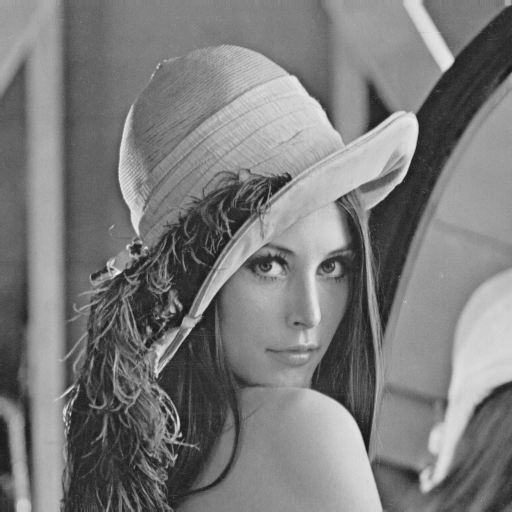
\includegraphics[width=\textwidth]{images/lena-y_128.png}
            \subcaption{$128$ levels}
        \end{subfigure}
        \hfill
        \begin{subfigure}[c]{0.3\textwidth}
            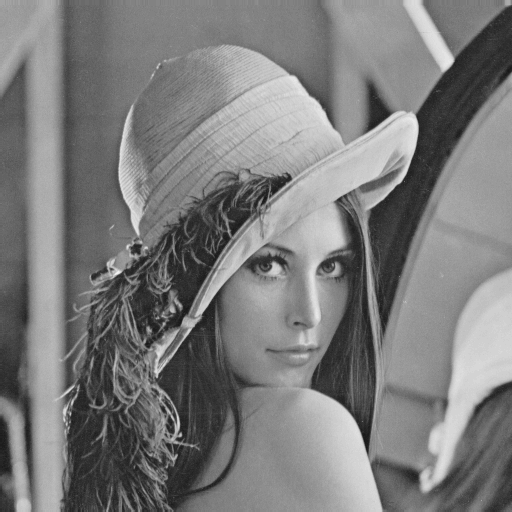
\includegraphics[width=\textwidth]{images/lena-y_64.png}
            \subcaption{$64$ levels}
        \end{subfigure}
        \hfill
        \begin{subfigure}[c]{0.3\textwidth}
            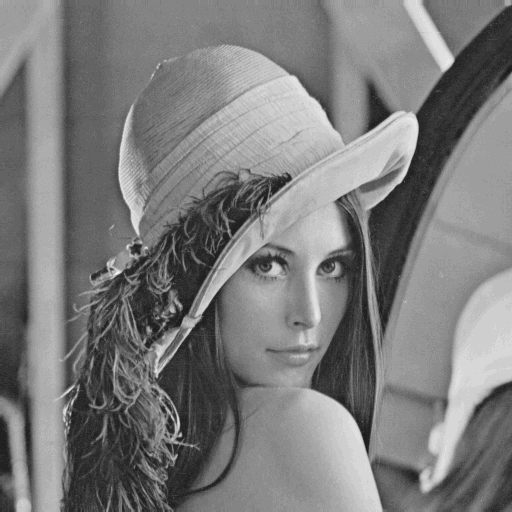
\includegraphics[width=\textwidth]{images/lena-y_32.png}
            \subcaption{$32$ levels}
        \end{subfigure}
        \hfill
        \begin{subfigure}[c]{0.3\textwidth}
            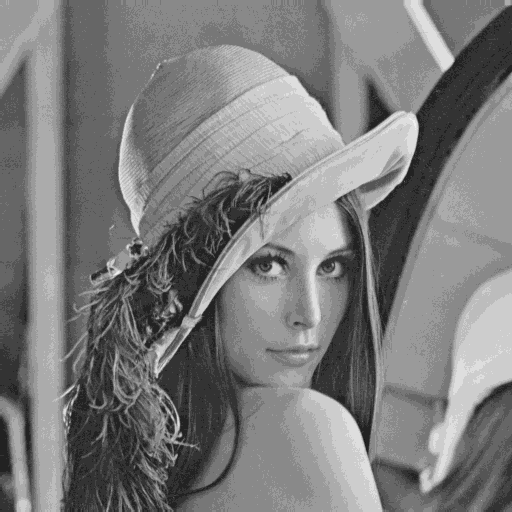
\includegraphics[width=\textwidth]{images/lena-y_16.png}
            \subcaption{$16$ levels}
        \end{subfigure}
        \hfill
        \begin{subfigure}[c]{0.3\textwidth}
            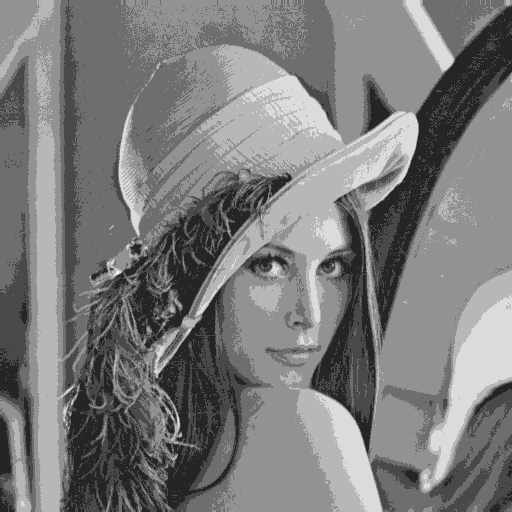
\includegraphics[width=\textwidth]{images/lena-y_8.png}
            \subcaption{$8$ levels}
        \end{subfigure}
        \hfill
        \begin{subfigure}[c]{0.3\textwidth}
            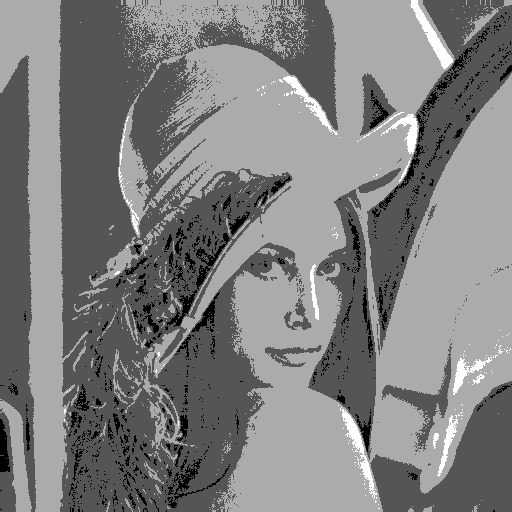
\includegraphics[width=\textwidth]{images/lena-y_4.png}
            \subcaption{$4$ levels}
        \end{subfigure}
        \hfill
        \begin{subfigure}[c]{0.3\textwidth}
            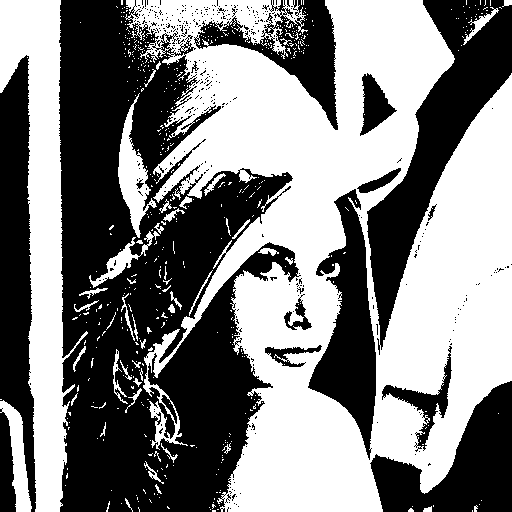
\includegraphics[width=\textwidth]{images/lena-y_2.png}
            \subcaption{$2$ levels}
        \end{subfigure}
        \caption{Uniform quantization for a different number of target grayscale levels.}
        \label{fig:quantization}
    \end{figure}

\section{Filtering}
In this task, two different filters had to be applied to the gold-text image. Figure \ref{fig:5x5} shows the magnitude of the frequency response of the first $5 \times 5$ separable 2D filter. To compute the frequency response, the matlab function freqz2() was used. If no output arguments are specified, it produces a mesh plot of the two-dimensional magnitude frequency response. The filter was then applied to the gold-text image by using the imfilter() matlab function, setting the 'conv' parameter to apply the filter using convolution. 
\begin{figure}
    \centering
    \begin{subfigure}[c]{0.49\textwidth}
        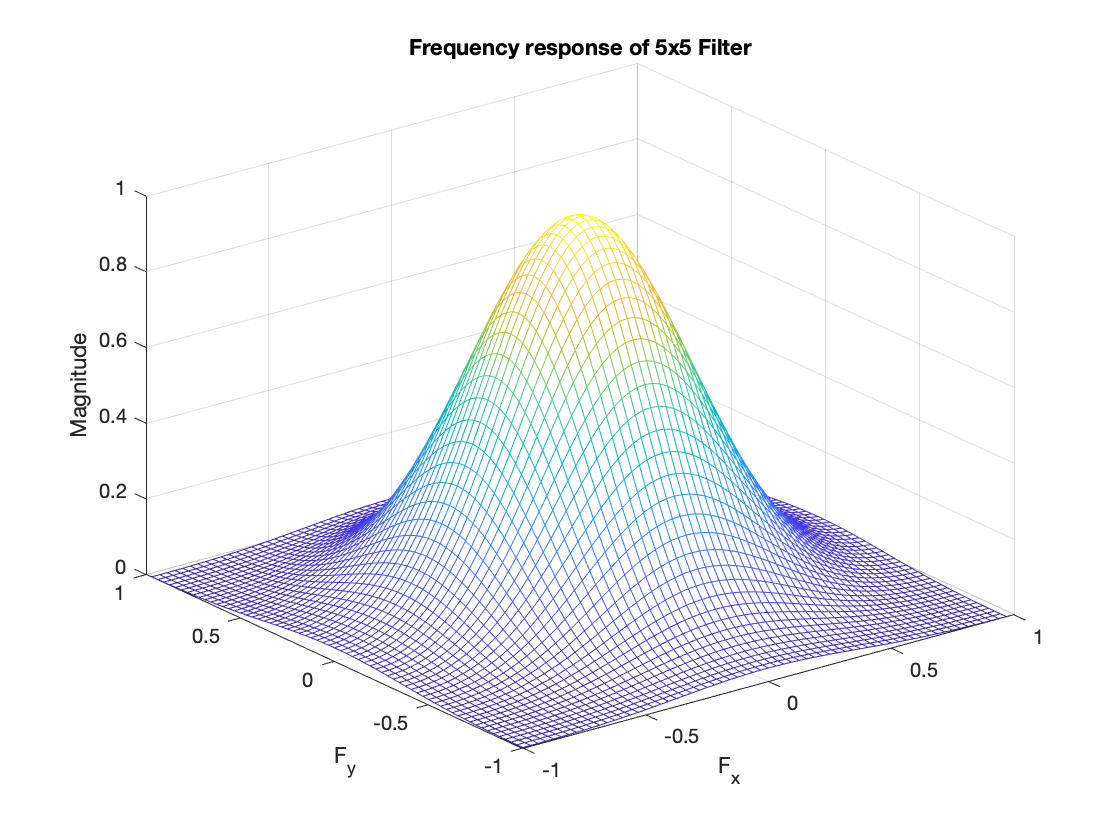
\includegraphics[width=\textwidth]{images/freq_resp_5x5.png}
        \subcaption{Frequency response of $5 \times 5$ filter}
    \end{subfigure}
    \hfill
    \begin{subfigure}[c]{0.49\textwidth}
        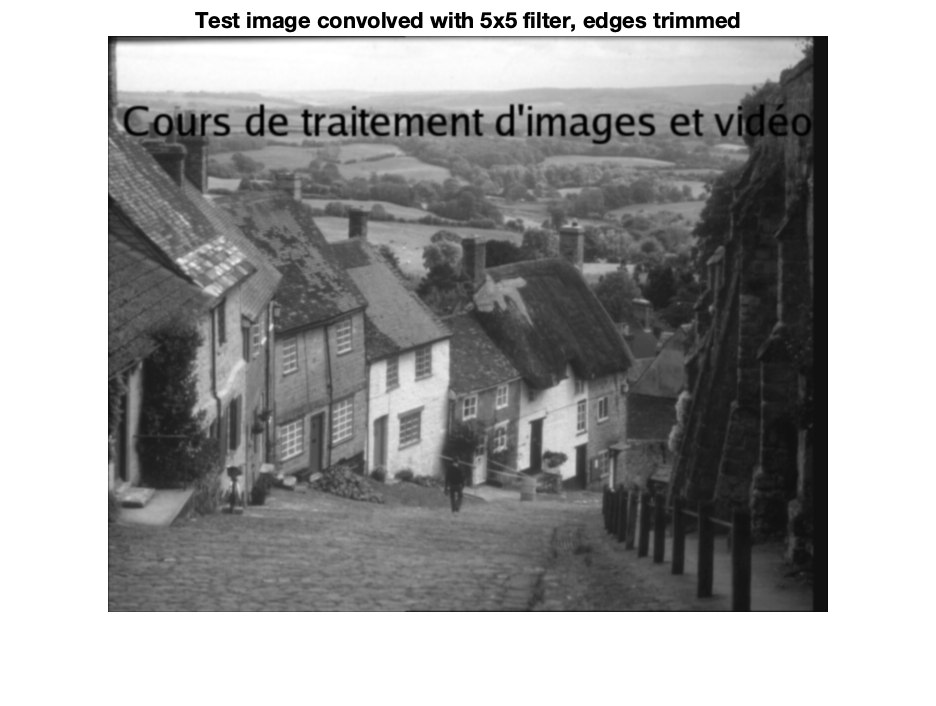
\includegraphics[width=\textwidth]{images/gold_text_filtered.png}
        \subcaption{$5 \times 5$ filter applied to gold-text image}
    \end{subfigure}
    \caption{Analysis of  $5 \times 5$ filter.}
    \label{fig:5x5}
\end{figure}
On the other hand, you can observe the frequency response and its application to the gold-text image through convolution of the $3 \times 3$ filter in Figure \ref{fig:3x3}.
\begin{figure}
    \centering
    \begin{subfigure}[c]{0.49\textwidth}
        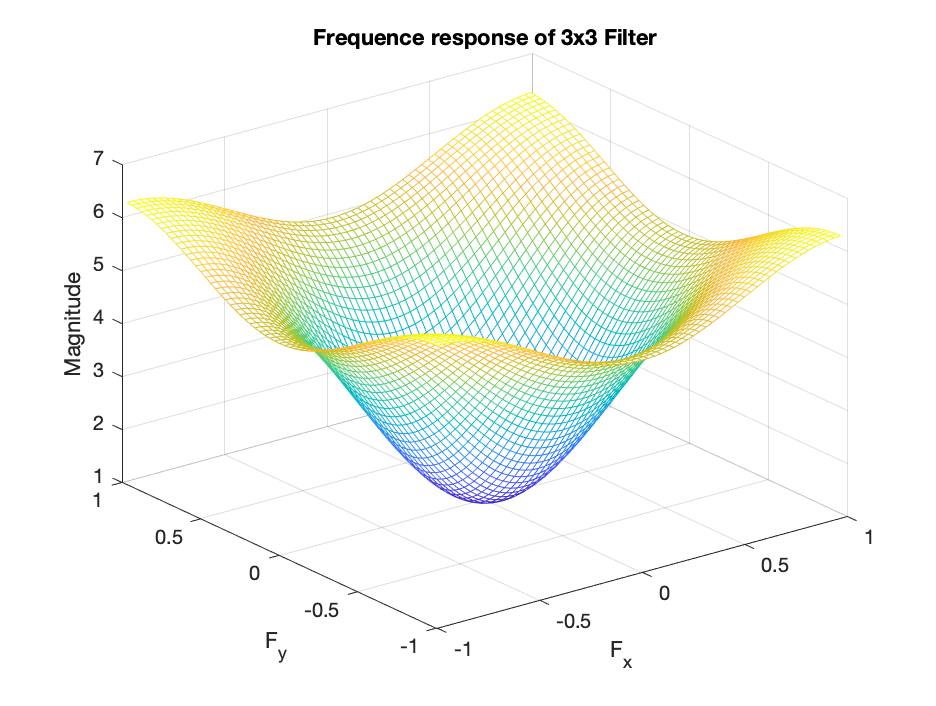
\includegraphics[width=\textwidth]{images/freq_resp_3x3.png}
        \subcaption{Frequency response of $3 \times 3$ filter}
    \end{subfigure}
    \hfill
    \begin{subfigure}[c]{0.49\textwidth}
        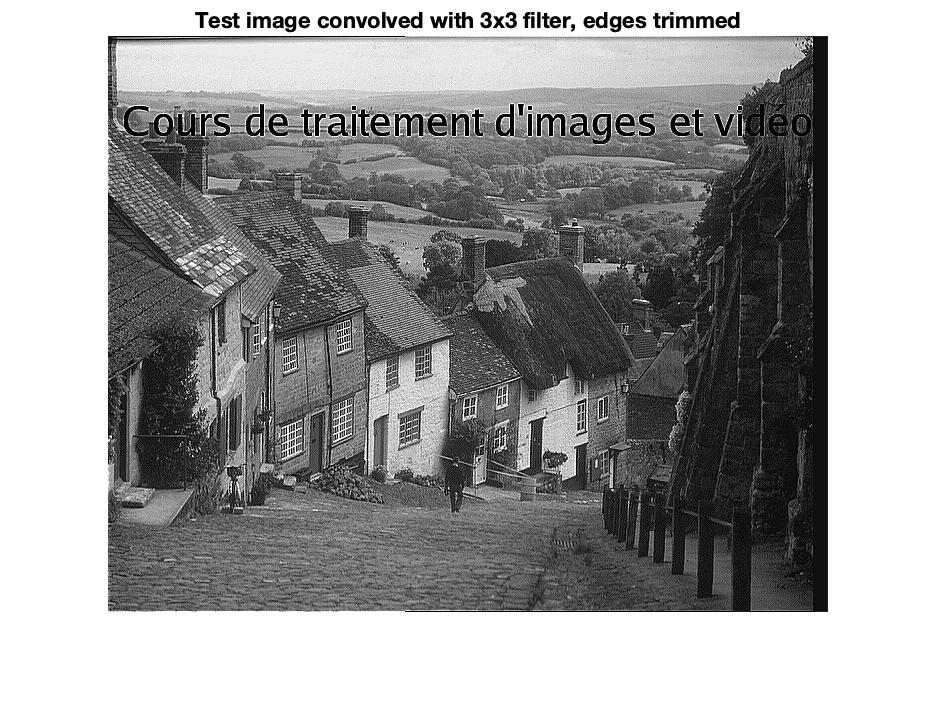
\includegraphics[width=\textwidth]{images/gold_text_filtered2.png}
        \subcaption{$3 \times 3$ filter applied to gold-text image}
    \end{subfigure}
    \caption{Analysis of  $3 \times 3$ filter.}
    \label{fig:3x3}
\end{figure}

The frequency response plots clearly visualize that, that the $5\times5$ filter is a low pass pass filter (shape of a Gaussian filter) while the $3 \times 3$ filter functions as a high pass filter. Thus, the gold text image is smoothed when applying the $5 \times 5$ filter, while contours are sharpened after applying the $3 \times 3$ filter (especially visible in the contours of the letters).

\section{Correlation}
For the fourth task, we were asked to detect a template pattern in an image using correlation. Since
\begin{equation*}
    \phi_{xy}(k, l) = x(-k, -l)**y(k, l),
\end{equation*}
we can express correlation through convolution. In particular, the template pattern was flipped from left to right using the matlab fliplr() function and was then applied to the target image using the conv2() function (which returns the two-dimensional convolution of two matrices) for, both, spatial and frequency (obtained through fft2(), which returns the two-dimensional Fourier transform of a matrix using a fast Fourier transform algorithm) domain. Note that, both, template and image were shifted to range from $-128$ to $127$. The maximum response location for the pattern resulting from the different correlation operations can be seen in Figure \ref{fig:correlation}. We can clearly see that the suggested position of the letter g better matches the true position when correlation is performed in the frequency domain.
\begin{figure}
    \centering
    \begin{subfigure}[c]{0.49\textwidth}
        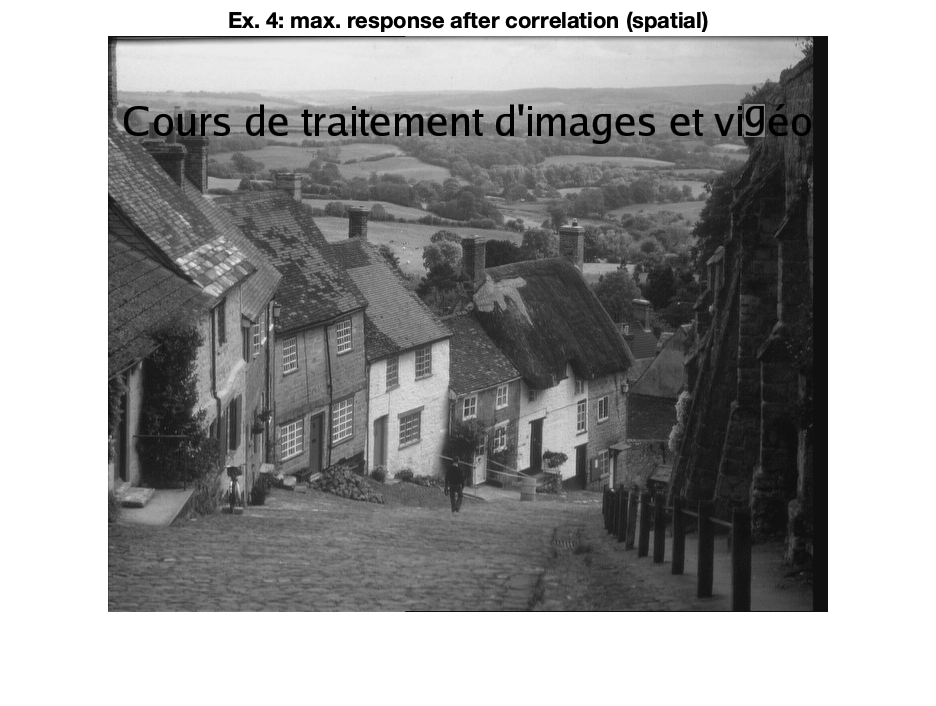
\includegraphics[width=\textwidth]{images/corr_spatial.png}
        \subcaption{Spatial domain}
    \end{subfigure}
    \hfill
    \begin{subfigure}[c]{0.49\textwidth}
        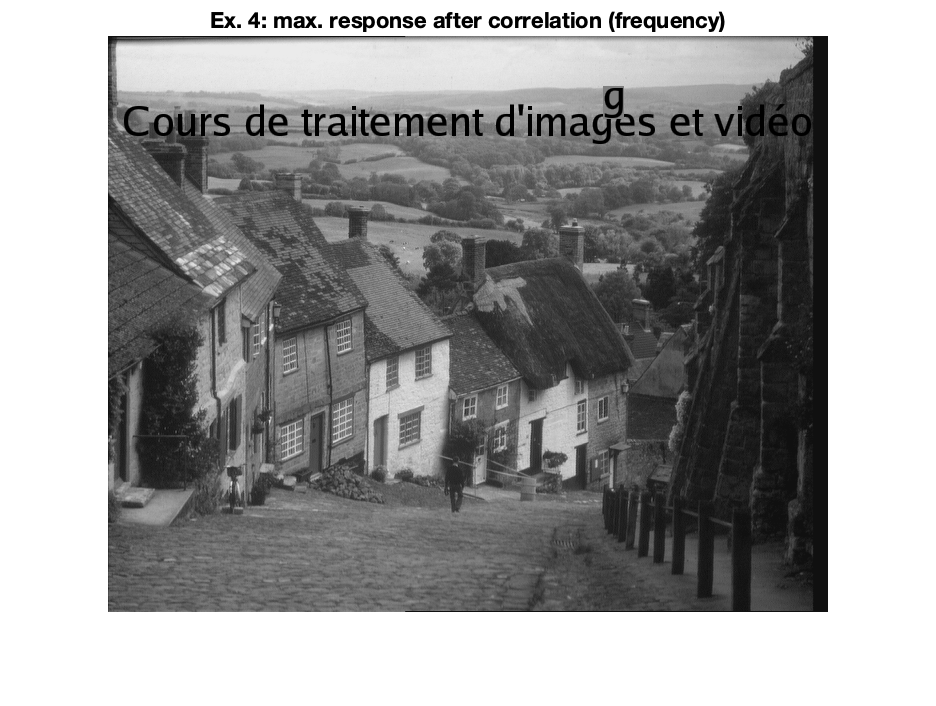
\includegraphics[width=\textwidth]{images/corr_freq.png}
        \subcaption{Frequency domain}
    \end{subfigure}
    \caption{Max. response location after correlation of source image and target pattern (letter g).}
    \label{fig:correlation}
\end{figure}

This was followed by applying uniform random noise to the image with standard deviations of $\sigma \in \{5, 10, 25, 40, 50\}$, ranging from $-128$ to $127$, again. The respective results after applying the correlation operator between the noisy image and the target pattern can be seen in Figure \ref{fig:correlation_noise}. The results clearly show that the correlation operation is highly sensitive to noise as the proposed position of the pattern strongly varies from the actual position and also across the different noise levels.

\begin{figure}
    \centering
    \begin{subfigure}[c]{0.3\textwidth}
        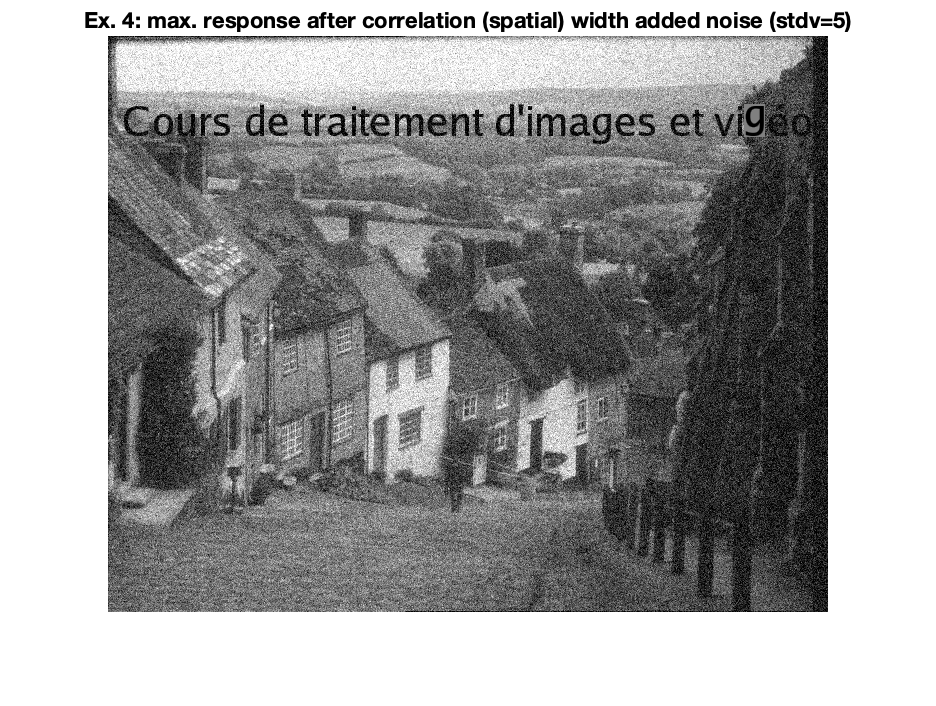
\includegraphics[width=\textwidth]{images/corr_spatial_noise_5.png}
        \subcaption{$\sigma = 5$}
    \end{subfigure}
    \begin{subfigure}[c]{0.3\textwidth}
        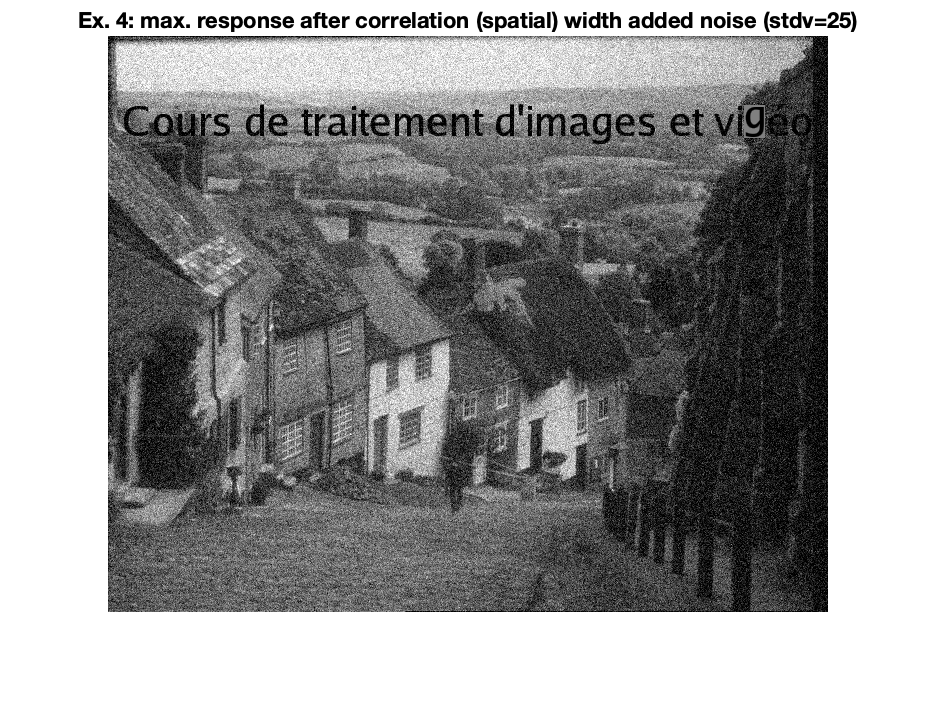
\includegraphics[width=\textwidth]{images/corr_spatial_noise_25.png}
        \subcaption{$\sigma = 25$}
    \end{subfigure}
    \begin{subfigure}[c]{0.3\textwidth}
        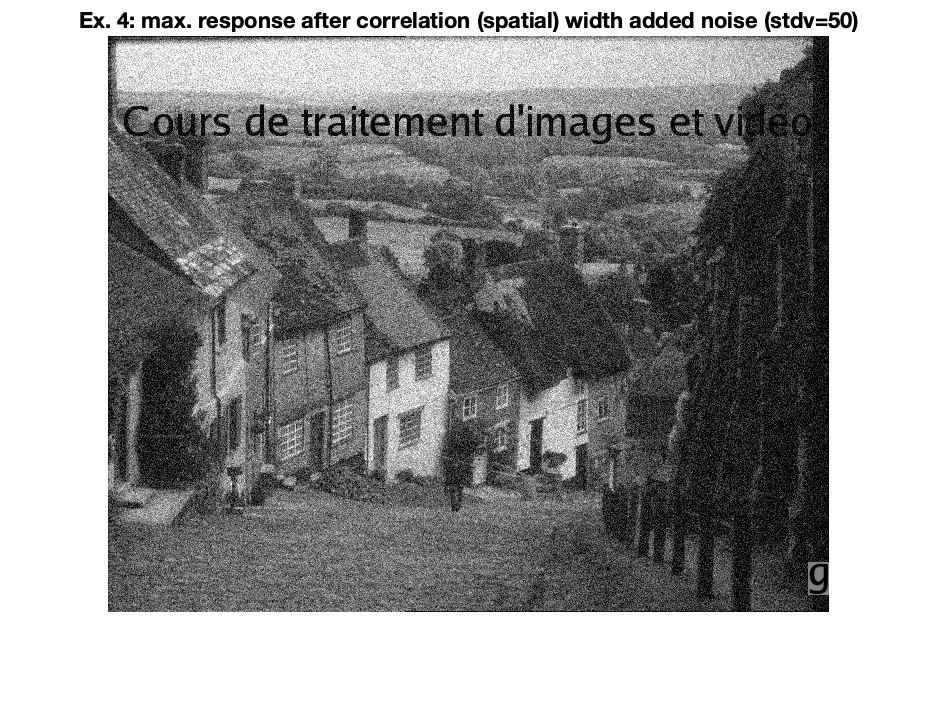
\includegraphics[width=\textwidth]{images/corr_spatial_noise_50.png}
        \subcaption{$\sigma = 50$}
    \end{subfigure}
    \caption{Max. response location after correlation of source image + uniform noise with different standard deviations and target pattern (letter g).}
    \label{fig:correlation_noise}
\end{figure}

Last but not least, matlab's normxcorr2() function was tested (although this was not required) and the respective result is shown in Figure \ref{fig:correlation_norm}. This function computes the normalized cross-correlation of the matrices template and search image. In this case, the location of the letter g is perfectly identified since normalized correlation is less sensitive to linear changes in illumination between the two images.

\begin{figure}
    \centering
    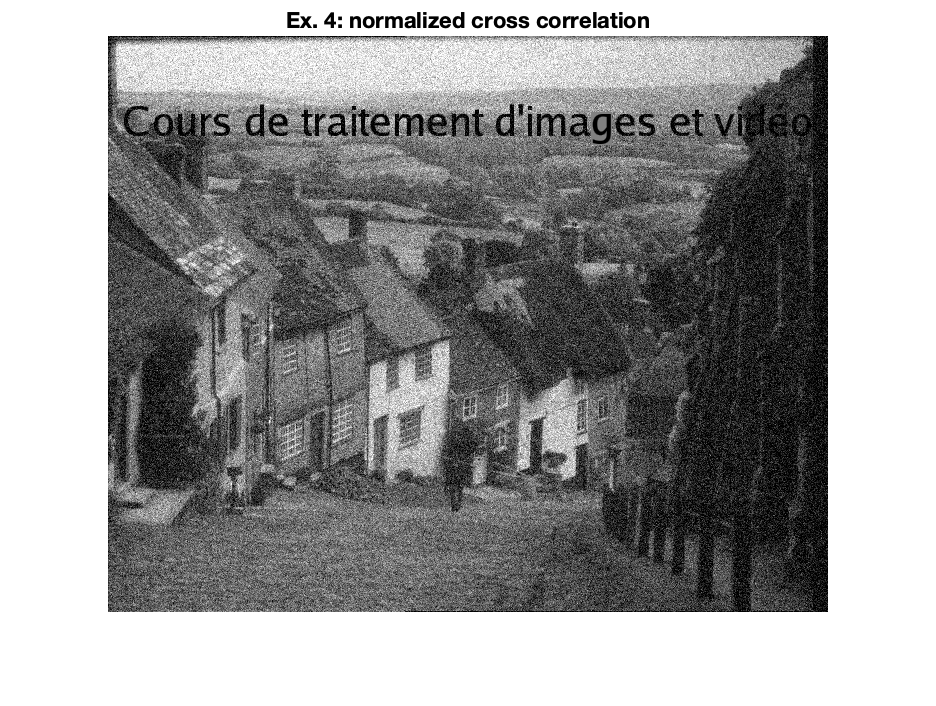
\includegraphics[width=0.6 \textwidth]{images/corr_normalized.png}
    \caption{Max. response location after normalized correlation between search image and target pattern.}
    \label{fig:correlation_norm}
\end{figure}

\section{Resampling}
This task was about downsampling an image by a factor of two and four. The respective results are shown in Figure \ref{fig:resample}. We observe Moiré patterns in the outer ring of both downsampled versions. Furthermore, numbers become unreadable in the factor 4 version. Last but not least, aliasing effects increase with increasing factor of the downsampled version.

\begin{figure}
    \centering
    \begin{subfigure}[c]{0.3\textwidth}
        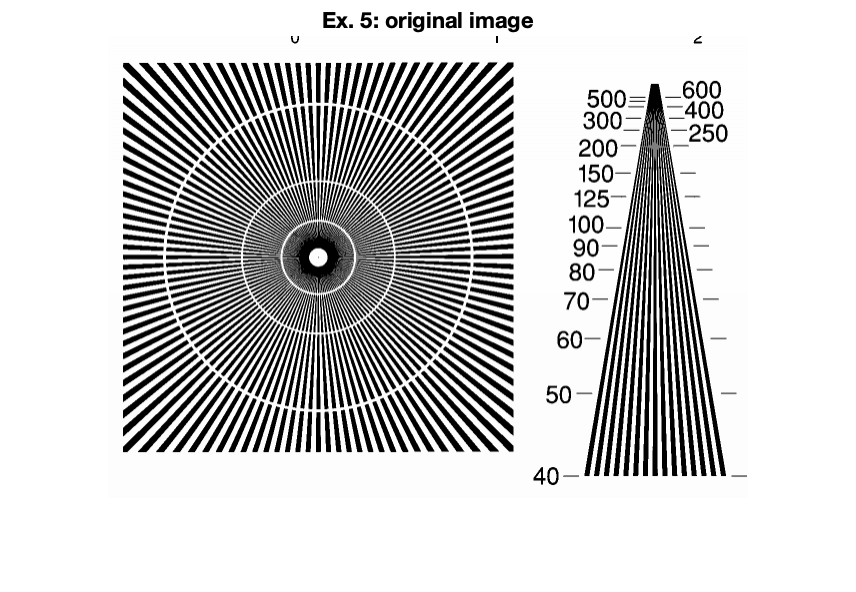
\includegraphics[width=\textwidth]{images/ex5.png}
        \subcaption{Original}
    \end{subfigure}
    \hfill
    \begin{subfigure}[c]{0.3\textwidth}
        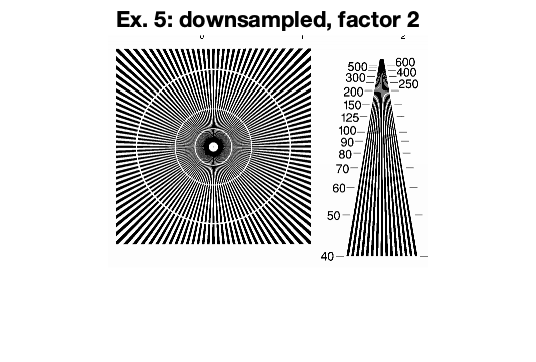
\includegraphics[width=\textwidth]{images/ex5_2.png}
        \subcaption{Factor 2}
    \end{subfigure}
    \hfill
    \begin{subfigure}[c]{0.3\textwidth}
        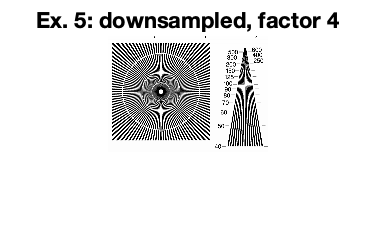
\includegraphics[width=\textwidth]{images/ex5_4.png}
        \subcaption{Factor 4}
    \end{subfigure}
    \caption{Downsampling an image by different factors}
    \label{fig:resample}
\end{figure}

\section{Phase and Magnitude of the 2DFT}
\begin{enumerate}
    \item The 2DFT was realized using matlab's fft2() function. It returns the two-dimensional Fourier transform of a matrix using a fast Fourier transform algorithm. Then, the imaginary part was deleted by only taking the real part using matlab's real() function, which returns the real part of a complex number. This was followed by applying matlabs ifft2() function, which returns the two-dimensional discrete inverse Fourier transform of a matrix using a fast Fourier transform algorithm. The steps were repeated on the original image, this time removing the real part and only keeping the imaginary part using matlab imag() function. The respective results can be seen in Figure \ref{fig:fourier}. We can see in Figure \ref{fig:fourier_real}, that the imaginary part seems to be important for reconstructing the orientation of the image. When removing the real part and visualizing the result, we obtain an image which looks like random noise. However, once we visualize the magnitude, we can observe enhanced edges and orientation ambiguities again. Thus, both, imaginary and real part seem to be important for fully reconstructing the signal. 
    \begin{figure}
    \centering
    \begin{subfigure}[c]{0.3\textwidth}
        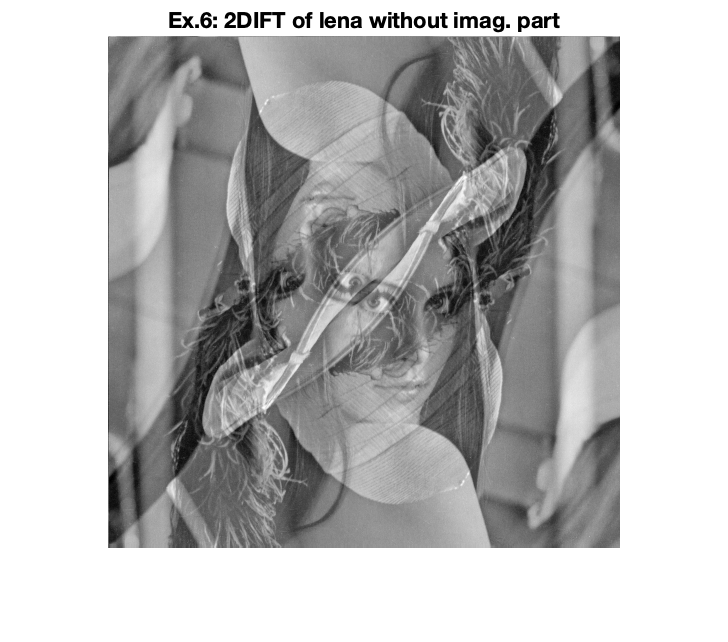
\includegraphics[width=\textwidth]{images/leana_real.png}
        \subcaption{Real part only}
        \label{fig:fourier_real}
    \end{subfigure}
    \begin{subfigure}[c]{0.3\textwidth}
        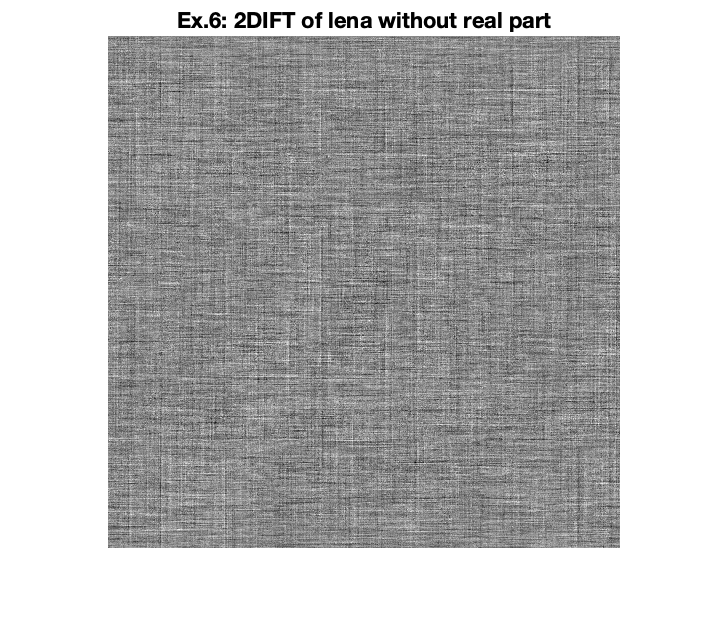
\includegraphics[width=\textwidth]{images/leana_imag.png}
        \subcaption{Imaginary part only}
    \end{subfigure}
    \begin{subfigure}[c]{0.3\textwidth}
        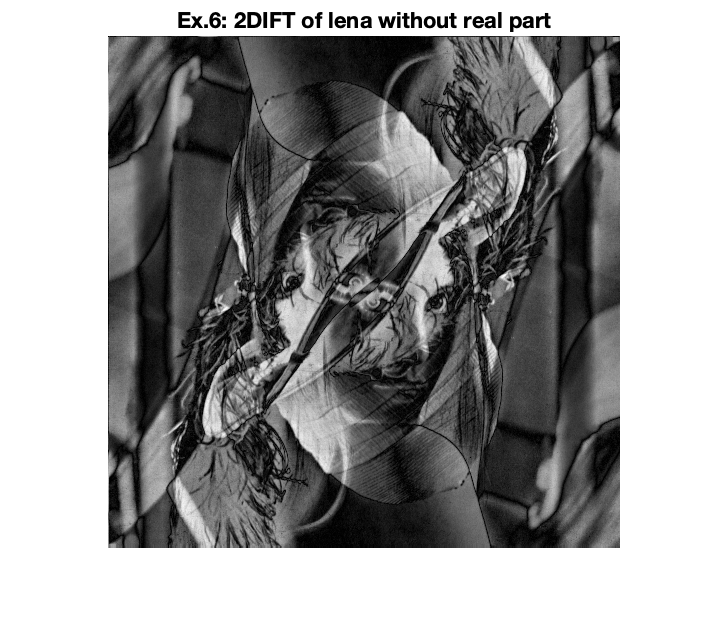
\includegraphics[width=\textwidth]{images/lena_imag_mag.png}
        \subcaption{Magnitude of imaginary part only}
    \end{subfigure}
    \caption{Removing real and imaginary part from 2DFT of input image and reconstructing result using 2DIFT.}
    \label{fig:fourier}
    \end{figure}
    \item For this task, the phase of the 2DFT was removed by only taking the magnitude (using matlab's abs()) of the signal, at first. Then, the 2DIFT was applied and the real part was visualized applying the logarithm to enhance small differences (cf. Figure \ref{fig:fourier_0phase}). We can observe, that the phase information is important for obtaining a reconstruction of the original signal which is visually correct for the human eye. In contrast, a magnitude of $1$ was achieved using the formula from the lecture, leading to the results shown in Figure \ref{fig:fourier_1mag}. In this case, the 2DIFT leads to a visually correct reconstruction of the input signal. Thus, the magnitude seems to be less important for the human eye.
    \begin{figure}
    \centering
    \begin{subfigure}[b]{0.4\textwidth}
        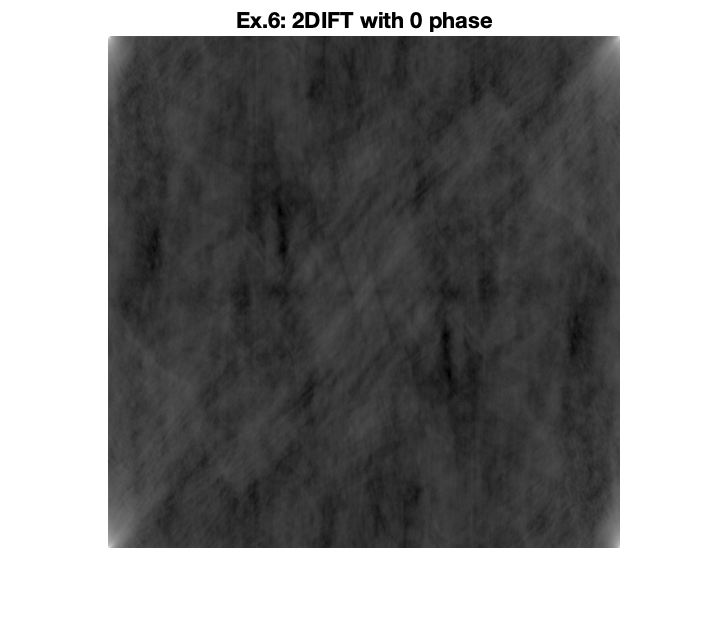
\includegraphics[width=\textwidth]{images/lena_0phase.png}
        \subcaption{Zero phase}
        \label{fig:fourier_0phase}
    \end{subfigure}
    \begin{subfigure}[b]{0.4\textwidth}
        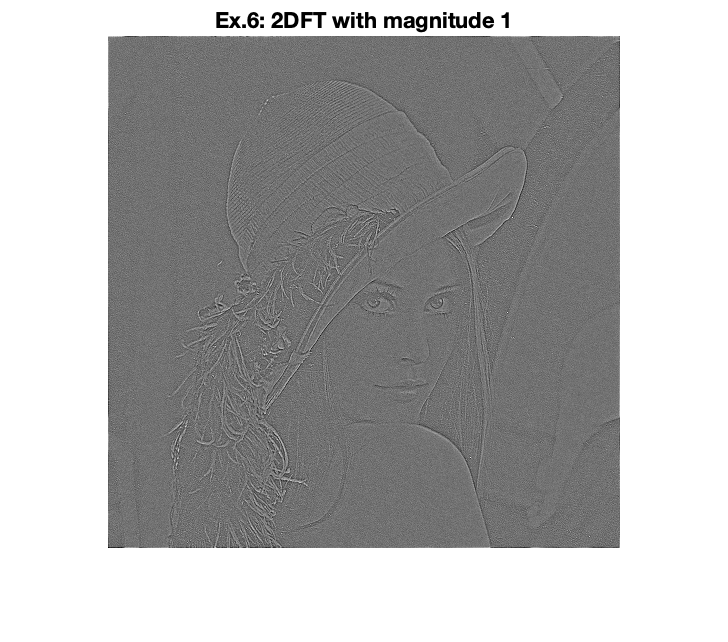
\includegraphics[width=\textwidth]{images/lena_1_mag.png}
        \subcaption{Magnitude of 1}
        \label{fig:fourier_1mag}
    \end{subfigure}
    \caption{Manipulating phase and magnitude in the Fourier domain.}
    \label{fig:fourier_mod}
    \end{figure}
\end{enumerate}

\section{Weber Law}
In this exercise, we were supposed to determine our Weber constant experimentally for different background intensities. To achieve this, the test image was created as described in the exercise. The intensities of $L1$ and $L2$ were then modified incrementally, bringing the intensities values closer step by step. In particular, this experiment was implemented in a way such that the participant could give a feedback on whether intensity differences between $L1$ and $L2$ were spotted or not. This was realized through console input, i.e. once the image is visualized, press any button to switch to console input. Press the key ``y" if you saw a difference between $L1$ and $L2$, otherwise hit ``n". Press ``Enter" afterwards. Depending on the participant's feedback, the values of $L1$ and $L2$ will be modified. \\
In order to advance quickly when there is still a large difference between $L1$ and $L2$, the intensity values are incremented/decremented by $10$ in case of a positive participant response. If an increment of $10$ is not possible anymore, we fall back to $5$ and then $1$ respectively. The same holds for the case if the participant did not notice a difference for an increment value $>1$. In this case, the previous intensity values are chosen again and a smaller increment value is selected. If the increment value is $1$ but no difference could be observed, the program terminates and the Weber constant is computed according to the formula in the exercise.\\
A distance of $50$ cm to the Retina display in ambient lighting were kept constant for all conditions. Furthermore, in order to avoid focusing on the boundary between $L1$ and $L2$, eyes were closed before each new condition.
\begin{enumerate}
    \item Cf. implementation
    \item First, $L_b=10, L1=100, L2=150$ was chosen resulting in a Weber constant of $0.016129$. $L_b=10, L1=230, L2=250$ resulted in a Weber constant of $0.017937$ and $L_b=10, L1=30, L2=70$ in $0.040816$.
    \item For $L_b = 200$, the following configurations were tested: $L_b=200, L1=100, L2=150$ which lead to a Weber constant of $0.016129$, $L_b=200, L1=230, L2=250$ resulting in $0.0083682$ and  $L_b=200, L1=30, L2=70$ in $0.040816$
\end{enumerate}
These results indicate that for this experiment, the intensity values of $L1$ and $L2$ seem to have had an influence on the minimal perceivable intensity difference. The Weber constant stayed the same for the two combinations $L1=100, L2=150$ and $L1=30, L2=70$ while the background $L_b$ changed. Only for $L1=230, L2=250$, a change was observable when $L_b$ changed. We obtain a larger Weber constant for $L_b = 10$, meaning that the difference between $L1$ and $L2$ at the point when no difference could be observed anymore was larger than for $L_b=200$. This seems to be a reasonable result since the strong contrast of $L_b$ to $L1$ and $L2$ makes $L1$ and $L2$ appear brighter and distracts from the contrast between $L1$ and $L2$, making these intensity values appear more similar. \\
However, no effect could be detected for the other conditions. Different confounding and extraneous variables, e.g. actual lighting condition, eye sight and concentration of participant, carry-over and sequence effects, etc. could have been the reason for this outcome. Thus, in order to obtain representative results, one would have to take a lot more consideration into this study design (e.g. randomizing conditions etc.).

\begin{figure}
    \centering
    \begin{subfigure}[c]{0.4\textwidth}
        
\includegraphics[width=\textwidth]{images/weber_10.png}
        \subcaption{$L_b = 10$}
    \end{subfigure}
    \begin{subfigure}[c]{0.4\textwidth}
        
\includegraphics[width=\textwidth]{images/weber_200.png}
        \subcaption{$L_b = 200$}
    \end{subfigure}
    \caption{Test images for $L1=230$, $L2=250$ for different values of $L_b$.}
    \label{fig:weber}
\end{figure}

\end{document}
